\chapter{Doxastic logic}

\section{Syntax and semantics}

Here we define the syntax and semantics of the logic \logicKDF{}, which
restricts the logic \logicK{}, as defined by van Ditmarsch and
French~\cite{french2009simulation}, to deal with only models and refinements of
models that are in \classKD{}.

% TODO - more motiviation

\begin{definition}[Language of \langF{}] % TODO - move to the K section
Given a finite set of agents $A$ and a set of propositional atoms $P$, the
language of \langF{} is defined by the following abstract syntax:

$$
\phi ::=    p \bnfalt
            \neg \phi \bnfalt
            \phi \land \phi \bnfalt
            \knows_a \phi \bnfalt
            \allrefs_a \phi
$$
where $a \in A$ and $p \in P$.
\end{definition}

Standard abbreviations include:
$\top ::= \phi \lor \neg \phi$;
$\bot ::= \neg \top$;
$\phi \lor \psi ::= \neg (\neg \phi \land \neg \psi)$;
$\phi \implies \psi ::= \neg \phi \lor \psi$;
and $\suspects_a \phi ::= \neg \knows_a \neg \phi$.
We use an abbreviation for the dual of the $\allrefs_a$ operator,
$\somerefs_a \phi ::= \neg \allrefs_a \neg \phi$.

We also use the cover operator $\covers_a \Gamma$, where $\Gamma$ is a finite
set of formulae, which is an abbreviation for 
$\covers_a \Gamma ::= \knows_a \bigvee_{\gamma \in \Gamma} \gamma \land
\bigwedge_{\gamma \in \Gamma} \suspects_a \gamma$. The cover operator is relied
on for our axiomatisation, in much the same way it is relied on for the
axiomatisation of \logicKiF{} presented by van Ditmarsch, French and
Pinchinat~\cite{french2010future}. % TODO - include citation for cover operator

\begin{definition}[Semantics of \logicCF]
Let $M = (S, R, V)$ be a doxastic model. The interpretation of $\phi \in
\logicKDF$ is defined inductively.

\begin{eqnarray*}
M_s &\entails& p \text{ iff } s \in V_p\\
M_s &\entails& \neg \phi \text{ iff } M_s \nentails \phi\\
M_s &\entails& \phi \land \psi \text{ iff } M_s \entails \phi \text{ and } M_s
\entails \psi\\
M_s &\entails& \knows_a \phi \text{ if for all } t \in S : (s, t) \in R_a \text{
implies } M_t \entails \phi\\
M_s &\entails& \allrefs_a \phi \text{ iff for all } M'_{s'} \in \classKD : M_s
\simulation_a M'_{s'} \text{ implies } M'_{s'} \entails \phi\\
\end{eqnarray*}
\end{definition}

The difference between \logicKF{} and \logicKDF{} is in the class of models that
they are interpreted over. It should be emphasised that the interpretation of
the refinement operator, $\allrefs_a$, varies for each logic, as the refinements
considered in the interpretation of the operator in \logicKDF{} must be taken
from the class of doxastic models, \classKD{}, whereas in \logicKF{} they may be
arbitrary Kripke models from \classK{}. It is for this reason that \logicKDF{}
is not a conservative extension of \logicKF{}. 

For example, the formula $\somerefs_a \knows_a \bot$ is valid in \logicKF{}, as
given any pointed Kripke model $M_s$, one can always form an $a$-refinement
$M'_{s'}$ of $M_s$ which simply removes all $a$-edges from $s$ in $M_s$, so that
$M'_{s'} \entails \knows_a \bot$. However $\somerefs_a \knows_a \bot$ is not
valid in \logicKDF{}, as all doxastic models have the serial property, and
hence there are no models in which $\knows_a \bot$ is true; therefore no
doxastic models can have a refinement where that is true.

\begin{lemma}
The logic \logicKDF{} is bisimulation invariant.
\end{lemma}

The proof for the bisimulation invariance of \logicKF{}, given by van Ditmarsch,
French and Pinchinat~\cite{french2010future} also applies to \logicKDF{}. 
% TODO - more explanation?

% TODO - examples

In previous work we gave an axiomatisation of the single-agent logic,
\logicKDiF{}, which relied upon a prenex normal form for the well-formed
formulae of \logicKDi{}. The prenex normal form prohibits modal operators
($\knows$ and $\suspects$) from appearing within other modal operators, and we
showed that all \logicKDi{} formulae are equivalent to a formula in prenex
normal form. The prenex normal form simplified the axiomatisation and proof of
soundness by avoiding complications that would arise due to the transitivity of
doxastic models.

We introduce a disjunctive normal form for the multi-agent logic \logicKD{},
which achieves the same purpose in terms of our axiomatisation as the prenex
normal form did for the single-agent \logicKD{}. In the multi-agent logic, it is
not possible to express all formulae in a form which prohibits nested modal
operators as in the prenex normal form, however it is possible to prohibit the
modal operators belonging to an agent $a$ (i.e. $\knows_a$ and $\suspects_a$)
from appearing directly within the scope of another modal operator belonging to
$a$. This allows us to avoid complications due to transitivity in our proof of
soundness for our axiomatisation of \logicKDF{}, in much the same way that
prenex normal form did for the axiomatisation of \logicKDiF{}.

\begin{definition}[Disjunctive normal form]
A formula in $a$-disjunctive normal form is defined by the following abstract syntax:

\begin{eqnarray*}
\alpha &::=& \delta \bnfalt \alpha \lor \alpha\\
\delta &::=& \pi \bnfalt \knows_b \gamma_b \bnfalt \suspects_b \gamma_b \bnfalt
\delta \land \delta\\
\end{eqnarray*}

Where $\pi$ stands for a propositional formula, $b \in A - \{a\}$, and
$\gamma_b$ stands for a formula in $b$-disjunctive normal form.

A formula in disjunctive normal form is defined by the following abstract syntax:

\begin{eqnarray*}
\alpha &::=& \delta \bnfalt \alpha \lor \alpha\\
\delta &::=& \pi \bnfalt \knows_a \gamma_a \bnfalt \suspects_a \gamma_a \bnfalt
\delta \land \delta\\
\end{eqnarray*}

Where $\pi$ stands for a propositional formula, $a \in A$, and $\gamma_a$
stands for a formula in $a$-disjunctive normal form.
\end{definition}

\begin{lemma}\label{kd45-dnf-equivalences}
We have the following equivalences in \logicKD{}:

\begin{eqnarray*}
\knows_a (\pi \lor (\alpha \land \knows_a \beta)) &\iff& (\knows_a (\pi \lor \alpha)
\land \knows_a \beta) \lor (\knows_a \pi \land \neg \knows_a \beta)\\
\knows_a (\pi \lor (\alpha \land \suspects_a \beta)) &\iff& (\knows_a (\pi \lor \alpha)
\land \suspects_a \beta) \lor (\knows_a \pi \land \neg \suspects_a \beta)
\end{eqnarray*}
\end{lemma}

This is proven by Meyer and van der Hoek~\cite{meyer2004epistemic} for
\logicSi{}, however the same proof also applies to \logicKD{}.

Meyer and van der Hoek remarked that the only use of the reflexivity axiom of
\logicS{}, {\bf T}, in the proof, is in the form of the theorems $\proves \knows
\knows \phi \implies \knows \phi$, and $\proves \knows \neg \knows \phi \implies
\neg \knows \phi$. Therefore the proof holds for any logic which replaces {\bf
T} with axioms entailing both of these properties. Both of these properties are
obviously valid in \logicKD{}, and therefore the proof by Meyer and van der
Hoek~\cite{meyer2004epistemic} applies to this result.

\begin{lemma}\label{kd45-dnf}
Every well-formed formula of \logicKD{} is equivalent to a formula in
disjunctive normal form.
\end{lemma}

\begin{proof}
We use a proof similar to the proof for prenex normal form, given by Meyer and
van der Hoek~\cite{meyer2004epistemic}.

Let $\phi$ be a well-formed formula of \logicKD{}. We proceed by induction on
the structure of $\phi$, with the induction hypothesis that every strict
subformula of $\phi$ is equivalent to a formula in disjunctive normal form.

Suppose that $\phi$ is a proposition. Then we are done; $\phi$ is in disjunctive
normal form.

Suppose that $\phi = \neg \alpha$. Then by the induction hypothesis, $\alpha$ is
equivalent to some $\alpha'$ in disjunctive normal form. We can use an inductive
argument, over $\alpha'$, to show that De Morgan's law can be repeatedly applied
to $\alpha'$ until the negation is pushed inwards, so that the only negations
are applied to propositional formulae (the result of which is a propositional
formula), thus yielding a formula equivalent to $\phi$. The result of this
process is a formula in disjunctive normal form. % TODO - more detail

Suppose that $\phi = \alpha \land \beta$. Then by the induction hypothesis, $\alpha$
and $\beta$ are equivalent to some $\alpha'$ and $\beta'$ in disjunctive normal
form. We note that we can equivalently write $\phi$ as $\phi = \neg (\neg
\alpha' \lor \neg \beta')$. From our case for negation, we note that $\neg
\alpha'$ and $\neg \beta'$ are equivalent to some $\alpha''$ and $\beta''$ in
disjunctive normal form. Given these, $\alpha'' \lor \beta''$ is also is
disjunctive normal form. Thus we can use our case for negation once again to
note that $\phi = \neg \alpha'' \lor \beta''$ is equivalent to some $\phi''$ in
disjunctive normal form.

Suppose that $\phi = \knows_a \psi$. Then by the induction hypothesis, $\psi$ is
equivalent to some $\psi'$ in disjunctive normal form. Suppose that $\psi'$ is
not in $a$-disjunctive normal form (otherwise we are done). Then $\psi'$
contains some conjunct of the form $\knows_a \beta$ or $\suspects_a \beta$. Thus
we can rewrite $\psi'$ as $\psi' = \pi \lor (\alpha \land \knows_a \beta)$. By
Lemma \ref{kd45-dnf-equivalences}, we get that $\phi \equiv (\knows_a (\pi \lor
\alpha) \land \knows_a \beta) \lor (\knows_a \pi \land \neg \knows_a \beta)$. We
can use the other equivalence from Lemma \ref{kd45-dnf-equivalences} in the case
that $\phi = \suspects_a \psi$.

Proceeding in this fashion we may move all conjuncts of $\psi'$ containing an
$a$-modality to the outside, so that they are conjuncts of $\phi$, thus
obtaining a formula in disjunctive normal form. % TODO - Make clearer
\end{proof}

\begin{definition}[Cover disjunctive normal form]\label{kd45-cdnf}
A formula in $a$-cover disjunctive normal form is defined by the following
abstract syntax:

$$
\alpha ::= \pi \land \bigwedge_{b \in A - \{a\}} \covers_b \Gamma_b \bnfalt
\alpha \lor \alpha
$$

Where $\pi$ stands for a propositional formula, and $\Gamma_b$ stands for a
finite, non-empty set of formulae in $b$-cover disjunctive normal form.

A formula in cover disjunctive normal form is defined by the following abstract
syntax:

$$
\alpha ::= \pi \land \bigwedge_{a \in A} \covers_a \Gamma_a \bnfalt
\alpha \lor \alpha
$$

Where $\pi$ stands for a propositional formula, and $\Gamma_a$ stands for a
finite, non-empty set of formulae in $a$-cover disjunctive normal form.
\end{definition}

\begin{lemma}
Every well-formed formula of \logicKD{} is equivalent to a formula in
cover disjunctive normal form.
\end{lemma}

\begin{proof}
Let $\phi$ be a \logicKD{} formula.  Without loss of generality, we may assume
that $\phi$ is in disjunctive normal form (by Lemma \ref{kd45-dnf}). We use an
inductive argument over the structure of $\phi$ to show that it can be converted
into cover disjunctive normal form.

The base case is where $\phi$ is a disjunctive normal formula containing no
modal operators. Then $\phi$ is simply a propositional formula. We can add
vacuous cover operators of the form $\covers_a \{\top\}$ for each $a \in A$.

Suppose that $\phi$ contains conjuncts of the form $\knows_a \gamma$ or
$\suspects_a \gamma$, where $\gamma$ is an $a$-disjunctive normal formula. By
the induction hypothesis, $\gamma$ is equivalent to some cover disjunctive
normal formula. We note that since $\gamma$ is an $a$-disjunctive normal
formula, any $a$-cover operator at the top-level of the equivalent cover
disjunctive normal formula must be vacuous. Therefore the $a$-cover operator may
be removed, yielding a formula in $a$-cover disjunctive normal form.

We can then convert the modal terms using the equivalences $\knows_a \gamma
\equiv \covers_a \{\gamma\}$ and $\suspects_a \gamma \equiv \covers_a \{\gamma,
\top\}$. We can add vacuous cover operators of the form $\covers_a \{\top\}$ for
any agent $a \in A$ which is not represented in our disjunct. We note that each
resulting set of formulae applied to a cover operator is non-empty.

An inductive argument can be used to show that we can collapse the resulting
conjunction of cover operators so that each agent is represented by a cover
operator only once. We use the following equivalence to achieve this.

$$
\covers_a \Gamma \land \covers_a \Gamma' \equiv 
\covers_a \big( 
\{ \gamma \land \bigvee_{\gamma' \in \Gamma'} \gamma' \mid \gamma \in \Gamma \}
\cup
\{ \gamma' \land \bigvee_{\gamma \in \Gamma} \gamma \mid \gamma' \in \Gamma' \}
\big)
$$

We note that as each of the $\gamma \in \Gamma$ and $\gamma' \in \Gamma'$ are
$a$-cover disjunctive normal formulae, a method similar to that used in the
proof of Lemma \ref{kd45-dnf} can be used to yield $a$-cover disjunctive normal
formulae that are equivalent to conjunctions and disjunctions of these formulae.
We note that each resulting set of formulae applied to a cover operator is
non-empty.

Repeating this for each disjunct in our original formula leaves us with a
formula in cover logic disjunctive normal form.
\end{proof}

The cover logic prenex normal form will be used in our completeness proofs.

\begin{lemma}\label{kd45-successors}
If $\phi$ is a formula in $a$-disjunctive normal form, and $M_s$ is a doxastic
model such that $M_s \entails \phi$, then there exists a model $N_t$ such that
$N_t \entails \phi$ and $tR^N_a = R^N_at = \{t\}$.
\end{lemma}

\begin{proof}
Suppose that $\phi$ is an $a$-disjunctive normal formula, and that $M_s$ is a
doxastic model such that $M_s \entails \phi$. 

Let $t \notin S^M$ and $t \notin S^{N^\gamma}$ for every $\gamma \in \Gamma$.
Then we construct a doxastic model $N = (S^N, R^N, V^N)$ where:

\begin{eqnarray*}
S^N &=& \{t\} \cup S^M\\
R^N_a &=& \{(t, t)\} \cup R^M_a\\
R^N_b &=& \{(t, s') \mid s' \in sR^M_b\} \cup R^M_b \text{ for every $b \in A -
\{a\}$}\\
V^N(p) &=& \begin{cases}
\{t\} \cup V^M(p) & \text{if $s \in V^M(p)$}\\
V^M(p) & \text{otherwise}
\end{cases}
\end{eqnarray*}

We note that $tR^N_a = R^N_at = \{t\}$.

We must first show that $N$ is a doxastic model, and then that $N_t \entails
\phi$. The latter will be shown by proving that for every $s' \in tR^N_b$, the
state $N_{s'}$ is bisimilar to $M_{s'}$.

First we show that $N$ is a doxastic model. The relation $R^N_a$ consists of the
relation $R^M_a$, combined with the relationship $(t,t)$. The latter addition
ensures the serial property given the new element in $S^N$, and as there are no
other relationships involving $t$, its addition preserves the transitivity and
Euclideaness of $R^M_a$. Hence $R^N_a$ is serial, transitive and Euclidean.
As $R^M_b$ is serial for $S^M$, and $tR^M_b = sR^M_b \ne \emptyset$, then
$R^N_b$ is serial for $S^N$. The relation $R^N_b$ for $b \in A - \{a\}$ consists
of the relation $R^M_b$, combined with relationships from $t$ to all of the
successors of $s \in S^M$. As $R^M_b$ is transitive and Euclidean, the
additional relationships, which are simply duplicates of relationships starting
at $s$ from $R^M_b$, also satisfy transitivity and Euclideaness, therefore
$R^N_b$ is also transitive and Euclidean. Therefore $N$ is a doxastic model.

We next show that for every $b \in A - \{a\}$ and each successor $s' \in sR^M_b$
of $s$, the state $N_{s'}$ is bisimilar to $M_{s'}$. This is by the bisimulation
relation $\mathcal{R} = \{(s', s') \mid s' \in S^M \}$, mapping states in
$M$ to their corresponding states in $N$. This is clearly a bisimulation as the
only state in $S^N$ which is not in $S^M$ is $t$, and there are no edges leading
to $t$ from any state in $S^M$.

As $\phi$ is in $a$-disjunctive normal form, $\phi$ has the form $\phi =
\delta_1 \lor \cdots \lor \delta_m$, where each $\delta_i$ has the form
$\delta_i = \gamma_i1 \land \cdots \land \gamma_i{n_i}$, and each $\gamma_{ij}$ is
either a propositional formula, or has the form $\knows_b \psi$ or $\suspects_b
\psi$ for some $b \in A - \{a\}$.  As $M_s \entails \phi$, there exists some $i
= 1, \dots, m$ such that $M_s \entails \delta_i$. Therefore, for every $j = 1,
\dots, n_i$, we have that $M_s \entails \gamma_{ij}$. Suppose that
$\gamma_{ij}$ is a propositional formula. Then by construction $N_t$ has the
same valuation as $M_s$, and hence is equivalent under propositional formulae.
Therefore $N_t \entails \gamma_{ij}$.  Suppose instead that $\gamma_{ij} =
\suspects_b \psi$ for some $b \in A - \{a\}$ and some formula $\psi$. Then there
exists some $s' \in sR^M_b$ such that $M_{s'} \entails \psi$. From above, we
know that $N_{s'}$ is bisimilar to $M_{s'}$, and so by bisimulation invariance
we have that $N_{s'} \entails \psi$.  By construction, $s' \in sR^M_b = tR^N_b$,
and hence $N_t \entails \suspects_b \psi$. A similar argument can be used for
the case where $\gamma_{ij} = \knows_b \psi$. Hence for every $j = 1, \dots,
n_i$, we have that $N_t \entails \gamma_ij$.

Hence $N_t \entails \delta_i$ and so $N_t \entails \psi$.
\end{proof}

\section{Axiomatisation}

\begin{definition}[\axiomKDF]
The axiomatisation \axiomKDF{} is a substitution schema consisting of the
following axioms:

$$
\begin{array}{rl}
{\bf P} & \text{All propositional tautologies}\\
{\bf K} & \knows (\phi \implies \psi) \implies \knows \phi \implies \knows
\psi\\
{\bf D} & \knows \phi \implies \suspects \phi\\
{\bf 4} & \knows \phi \implies \knows \knows \phi\\
{\bf 5} & \suspects \phi \implies \knows \suspects \phi\\
{\bf RP} & \allrefs_a (\phi \implies \psi) \implies \allrefs_a \phi \implies
\allrefs_a \psi\\
{\bf RK} & \allrefs_a \alpha \iff \alpha \text{ where $\alpha$ is a
propositional formula}\\
{\bf RComm} & \somerefs_a \covers_b \Gamma \iff \covers_b \{\somerefs_a \gamma
\mid \gamma \in \Gamma\}\\ 
&\qquad\text{where $a \neq b$ and $\Gamma$ is a set of $b$-disjunctive normal formulae}\\
{\bf RDist} & \bigwedge_{b \in A} \somerefs_a \covers_b \Gamma_b \implies
\somerefs_a \bigwedge_{b \in A} \covers_b \Gamma_b\\
&\qquad\text{where $\Gamma_b$ is a set of $b$-disjunctive normal formulae for every $b \in A$}\\
{\bf RKD45} & \somerefs_a \covers_a \Gamma \iff \bigwedge_{\gamma \in \Gamma}
\suspects_a \somerefs_a \gamma\\
&\qquad\text{where $\Gamma$ is a non-empty set of $a$-disjunctive
normal formulae}\\
\end{array}
$$

Along with the rules:

$$
\begin{array}{rl}
{\bf MP} & \text{From $\proves \phi \implies \psi$ and $\proves \phi$, infer
$\proves \psi$}\\
{\bf NecK} & \text{From $\proves \knows_a (\phi \implies \psi)$ and $\proves
\knows_a \phi$, infer $\proves \knows_a \psi$}\\
{\bf NecR} & \text{From $\proves \allrefs_a (\phi \implies \psi)$ and $\proves
\allrefs_a \phi$, infer $\proves \allrefs_a \psi$}
\end{array}
$$
\end{definition}

\begin{lemma}\label{kd45-sound}
The axiomatisation \axiomKDF{} is sound in \logicKDF{}.
\end{lemma}

\begin{proof}
The soundness of the axioms {\bf P}, {\bf K}, {\bf D}, {\bf 4}, and {\bf 5} and the
rules {\bf MP} and {\bf NecK} can be shown by the same reasoning used to show
that they are sound in \logicKD{}. The soundness of the axioms {\bf RP} and {\bf
RK}, and the rule {\bf NecR} can be shown by the same reasoning used to how
that they are sound in the \logicKiF{}~\cite{french2010future}.

All that remains to be shown is the soundness of {\bf RKD45}, {\bf RComm}, and
{\bf RDist}.

\paragraph{RKD45}
Suppose that $M_s$ is a doxastic model such that $M_s \entails \bigwedge_{\gamma
\in \Gamma} \suspects_a \somerefs_a \gamma$, where $\Gamma$ is a non-empty set of
$a$-disjunctive normal formulae.

Then consider $\gamma \in \Gamma$. From $M_s \entails \suspects_a \somerefs_a
\gamma$, there exists a state $s^\gamma \in sR^M$ such that $M_{s^\gamma}
\entails \somerefs_a \gamma$. Therefore there exists a doxastic model
$N^\gamma_{t^\gamma} \refinement_a M_{s^\gamma}$, via some $a$-simulation
$\mathcal{R}^\gamma$, such that $N^\gamma_{t^\gamma} \entails \gamma$.

Without loss of generality we assume that each $N^\gamma$ is disjoint, and as
each $\gamma$ is an $a$-disjunctive normal formula, by Lemma
\ref{kd45-successors}, we may assume that $t^\gamma R^{N^\gamma}_a =
\{t^\gamma\}$.

Let $t \notin S^M$ and $t \notin S^{N^\gamma}$ for every $\gamma \in \Gamma$.
Then we construct a doxastic model $N = (S^N, R^N, V^N)$ where:

\begin{eqnarray*}
S^N &=& \{t\} \cup S^M \cup \bigcup_{\gamma \in \Gamma} S^{N^\gamma}\\
R^N_a &=& \{(t, t^\gamma) \mid \gamma \in \Gamma\} 
\cup \{(t^\gamma, t^{\gamma'}) \mid \gamma, \gamma' \in \Gamma\} 
\cup R^M_a
\cup \bigcup_{\gamma \in \Gamma} R^{N^\gamma}_a\\
R^N_b &=& \{(t, t') \mid t' \in sR^M_b\}
\cup R^M_b
\cup \bigcup_{\gamma \in \Gamma} R^{N^\gamma}_b \text{ for $b \in A - \{a\}$}\\
V^N(p) &=& 
\begin{cases}
\{t\} \cup V^M(p) \cup \bigcup_{\gamma \in \Gamma} V^{N^\gamma}(p) & \text{if $s
\in V^M(p)$}\\
V^M(p) \cup \bigcup_{\gamma \in \Gamma} V^{N^\gamma}(p) & \text{otherwise}
\end{cases}
\text{ for $p \in P$}
\end{eqnarray*}

\begin{figure}[H]
\begin{center} % TODO - better diagram
\scalebox{0.4}{
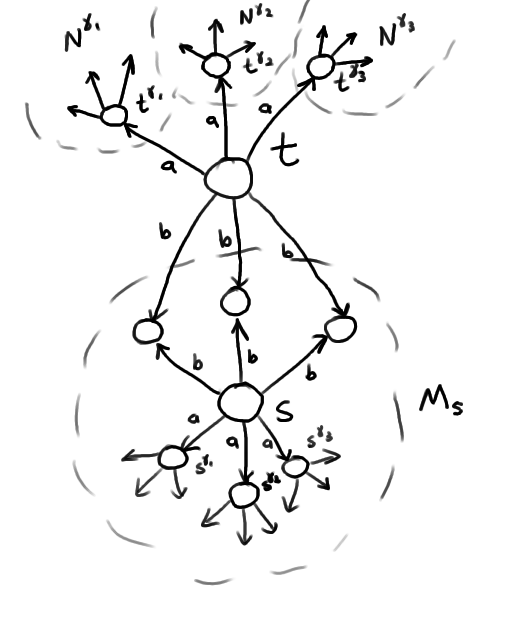
\includegraphics{diagram}
}
\caption{
The model $N$ is constructed by taking the model $M$ and the models $N^\gamma$
for every $\gamma \in \Gamma$, and connecting them with an extra node $t$. $t$
is connected via an $a$-edge to $t^\gamma$ from each of the $N^\gamma$, and is
also connected via a $b$-edge to each $b$-successor of $s$ in $M$.
}
\end{center}
\end{figure}

We must show that $N$ is a doxastic model, that $N_t$ is an $a$-refinement of
$M_s$, and that for every $t^\gamma \in tR^N_a$ we have that $N_{t^\gamma}
\entails \gamma$. The latter will be shown by proving that for every $\gamma \in
\Gamma$, the state $N_{t^\gamma}$ is bisimilar to $N^\gamma_{t^\gamma}$.

First we show that $N$ is a doxastic model. We must show two cases: that $R^N_a$
is serial, transitive and Euclidean, and that $R^N_b$ is also serial, transitive
and Euclidean, for every $b \in A - \{a\}$. As $M$ and each $N^\gamma$ are doxastic
models, the relations $R^M_c$ and $R^{N^\gamma}_c$ are serial, transitive and
Euclidean, for every $c \in A$. We observe that $S^N$ is a union of $\{t\}$,
$S^M$ and each $S^{N^\gamma}$. As $\Gamma$ is non-empty there is at
least one relationship $(t, t^\gamma)$ in $R^N_a$, therefore as $R^N_a$ also
contains $R^M_a$ and each $R^{N^\gamma}_a$, each of which are serial, then $R^N_a$
is also serial. Similarly, as $M$ is serial, $sR^M_b$ is non-empty, and so there
is at least one relationship $(t, t')$ where $t' \in sR^M_b$ in $R^N_b$;
therefore as $R^N_b$ also contains $R^M_b$ and $R^{N^\gamma}_b$, then $R^N_b$ is
also serial. To show the transitivity and Euclideaness of $R^N_a$, we first
observe that the relation can be considered in three independent parts; the
relationships between $t$ and $t^\gamma$, and between each $t^\gamma$; the
relation $R^M_a$; and the relations $R^{N^\gamma}_a$. The relation $R^M_a$ is
disjoint from the other relations, and so can be considered in isolation. By
hypothesis we have assumed that $t^\gamma R^{N^\gamma}_a = \{t^\gamma\}$, so as
there are no relationships from any $t^\gamma$ to a different state in
$S^{N^\gamma}$, we can also consider the each $R^{N^\gamma}_a$ separately from
the rest of $R^N_a$. We note that as $R^M_a$ and each $R^{N^\gamma}_a$ are
transitive and Euclidean, and as the remainder of the relation is essentially an
equivalence relation without the relationship $(t, t)$, it also has transitivity
and Euclideaness. Therefore $R^N_a$ is transitive and Euclidean. We can show
that $R^N_b$ is also transitive and Euclidean from the fact that $R^M_b$ and
each $R^{N^\gamma}_b$ is transitive and Euclidean, and otherwise disjoint from
each other, and the remainder of $R^N_b$ is simply a duplicate of relationships
from $s$ to its successors, then $R^N_b$ is also transitive and Euclidean.
Therefore $N$ is a doxastic model.

We next show that $N_t$ is an $a$-refinement of $M_s$. We construct an
$a$-simulation $\mathcal{R}$ from $N_t$ to $M_s$, where:

$$\mathcal{R} = \{(t, s)\} \cup \{(s', s') \mid s' \in S^M \} \cup \bigcup_{\gamma \in \Gamma} \mathcal{R}^\gamma$$

We must show that $\mathcal{R}$ satisfies {\bf atoms}, {\bf forth-$b$} for every
$b \in A$, and {\bf back-$b$} for every $b \in A - \{a\}$.

We note that, by construction, the valuation of $N$ matches the valuation of its
corresponding states in $M$ and each $N^\gamma$, and the valuation of $N_t$
matches that of $M_s$. Therefore $\mathcal{R}$ satisfies {\bf atoms}.

We next show that $\mathcal{R}$ satisfies {\bf forth-$b$} for every $b \in A$.
Let $b \in A$, $u \in S^N$ and $v \in S^M$ such that $(u, v) \in
\mathcal{R}$. Suppose that $(u, v) \in \mathcal{R}^\gamma$ for some $\gamma \in
\Gamma$. Then as $\mathcal{R}^\gamma$ is an $a$-simulation, it satisfies {\bf
forth-$b$} for every $b \in A$. Hence for every $u' \in uR^N_b$, there exists
some $v' \in vR^M_b$ such that $(u', v') \in \mathcal{R}^\gamma \subseteq
\mathcal{R}$. Suppose instead that $(u, v) = (s', s')$ for some $s' \in S^M$.
Then we note that $s'R^N_b = s'R^M_b$, and hence for every $s'' \in s'R^N_b$ we
have that $s'' \in s'R^M_b$, and that $(s'', s'') \in \mathcal{R}$. Finally suppose
that $(u, u') = (t, s)$. Then suppose that $b = a$. By construction, $tR^N_a =
\{t^\gamma \mid \gamma \in \Gamma\}$, and hence $v = t^\gamma$ for some $\gamma
\in \Gamma$. Hence we can take $s^\gamma \in sR^M_a$, and note that as
$\mathcal{R}^\gamma$ is an $a$-simulation from $M_{s^\gamma}$ to
$N^\gamma_{t^\gamma}$, we know that $(t^\gamma, s^\gamma) \in \mathcal{R}^\gamma
\subseteq \mathcal{R}$. Suppose that $b \neq a$. Then by construction, $tR^M_b =
sR^M_b$, hence for every $t' \in tR^M_b$, we have that $t' \in sR^M_b$, and
hence we know that $(t', t') \in \mathcal{R}$. Hence $\mathcal{R}$ satisfies
{\bf back-$b$} for every $b \in A$.

A similar argument to above shows that $\mathcal{R}$ satisfies {\bf forth-$b$}
for every $b \in A - \{a\}$.

Hence $\mathcal{R}$ is an $a$-simulation from $N_t$ to $M_s$. Thus $N_t
\refinement_a M_s$. 

We next show that for every $\gamma \in \Gamma$, we have that $N_{t^\gamma}
\entails \gamma$. As each $\gamma$ is an $a$-disjunctive normal formula, a
similar argument to that used in Lemma \ref{kd45-successors} can be used to show
that $N_{t^\gamma}$ is bisimilar to $N^\gamma_{t^\gamma}$ (as there are only
edges added going into $N_{t^\gamma}$, not coming out). Therefore, as for every
$\gamma \in \Gamma$ we have that $N^\gamma_{t^\gamma} \entails \gamma$, by
bisimulation invariance we also have that $N_{t^\gamma} \entails \gamma$. Hence
$N_t \entails \covers_a \Gamma$.

As $N_t \refinement_a M_s$, and $N_t \entails \covers_a \Gamma$ we therefore
have that $M_s \entails \somerefs_a \covers_a \Gamma$.

Conversely, suppose that $M_s \entails \covers_a \Gamma$. Then there exists a
doxastic model $N_t \refinement_a M_s$, via some $a$-simulation $\mathcal{R}$,
such that $N_t \entails \covers_a \Gamma$. From the definition of the cover
operator, this implies that $N_t \entails \knows_a \bigvee_{\gamma \in \Gamma}
\gamma \land \bigwedge_{\gamma \in \Gamma} \suspects_a \gamma$. In particular we
note that for every $\gamma \in \Gamma$, $N_t \entails \suspects_a \gamma$, and
so there exists some $t^\gamma \in tR^N_a$ such that $N_{t^\gamma} \entails
\gamma$. As $t^\gamma \in tR^N_a$, and $(t, s) \in \mathcal{R}$, by {\bf
forth-$a$} there exists some $s^\gamma \in sR^M_a$ such that $(t^\gamma, s^\gamma)
\in \mathcal{R}$. Hence $\mathcal{R}$ is also an $a$-simulation from
$N_{t^\gamma}$ to $M_{s^\gamma}$, and so $M_{s^\gamma} \entails \somerefs_a
\gamma$. As for every $\gamma \in \Gamma$ we have that $s^\gamma \in sR^M_a$, we
also have that $M_s \entails \suspects_a \somerefs_a \gamma$. Therefore we
finally have that $M_s \entails \bigwedge_{\gamma \in \Gamma} \suspects_a
\somerefs_a \gamma$.

Therefore {\bf RKD45} is sound.

\paragraph{RComm} Suppose that $M_s$ is a doxastic model such that $M_s
\entails \covers_b \{ \somerefs_a \gamma \mid \gamma \in \Gamma\}$, where $a \ne
b$ and $\Gamma$ is a set of $b$-disjunctive normal formulae. From the definition
of the cover operator, this implies that $M_s \entails \knows_b \bigvee_{\gamma
\in \Gamma} \somerefs_a \gamma \land \bigwedge_{\gamma \in \Gamma} \suspects_b
\somerefs_a \gamma$. In particular, we note that for every $\gamma \in \Gamma$,
there exists some $s^\gamma \in sR^M_b$ such that $M_{s^\gamma} \entails
\somerefs_a \gamma$.  Then there exists a doxastic model $N^\gamma_{t^\gamma}
\refinement_a M_{s^\gamma}$, via some $a$-simulation $\mathcal{R}^\gamma$, such
that $N^\gamma_{t^\gamma} \entails \gamma$. Without loss of generality, as
$\gamma$ is a $b$-disjunctive normal formula, we may assume that $t^\gamma
R^{N^\gamma}_b = \{t^\gamma\}$ (by Lemma \ref{kd45-successors}), and that the
$N^\gamma$ are disjoint.

Let $t$ be a state such that $t \notin S^{N^\gamma}$ for every $\gamma \in
\Gamma$. Then we construct a model $N = (S^N, R^N, V^N)$, where:

\begin{eqnarray*}
S^N &=& \{t\} \cup S^M \bigcup_{\gamma \in \Gamma} S^{N^\gamma}\\
R^N_b &=& \{(t, t^\gamma) \mid \gamma \in \Gamma\} \cup \{(t^\gamma,
t^{\gamma'}) \mid \gamma, \gamma' \in \Gamma\} \cup R^M_b \cup \bigcup_{\gamma
\in \Gamma} R^{N^\gamma}_b\\
R^N_c &=& \{(t, t') \mid t' \in sR^M_c\} \cup R^M_c \cup \bigcup_{\gamma \in
\Gamma} R^{N^\gamma}_c \text{ for $c \in A - \{b\}$}\\
V^N(p) &=& 
\begin{cases}
\{t\} \cup V^M(p) \cup \bigcup_{\gamma \in \Gamma} V^{N^\gamma}(p) & \text{if $s
\in V^M(p)$}\\
V^M(p) \cup \bigcup_{\gamma \in \Gamma} V^{N^\gamma}(p) & \text{otherwise}
\end{cases}
\text{ for $p \in P$}
\end{eqnarray*}

We note that $N$ is a doxastic model, by similar arguments as used in the proof
for {\bf RKD45}.

We next construct an $a$-simulation $\mathcal{R}$ from $N_t$ to $M_s$, where:

$$\mathcal{R} = \{(t, s)\} \cup \{(s', s') \mid s' \in S^M\} \cup \bigcup_{\gamma \in \Gamma} \mathcal{R}^\gamma$$

We note that $\mathcal{R}$ is an $a$-simulation, by similar arguments as used in
the proof for {\bf RKD45}. In particular, this means that $N_t \refinement_a
M_s$.

We also note that for every $\gamma \in \Gamma$ that $N_{t^\gamma} \bisim
N^\gamma_{t^\gamma}$, by similar arguments as used in the proof for {\bf RKD45}.
In particular, this means that as $N^\gamma_{t^\gamma} \entails \gamma$ that we
also have $N_{t^\gamma} \entails \gamma$, for every $\gamma \in \Gamma$.
Therefore $N_t \entails \covers_b \Gamma$.

Therefore $M_s \entails \somerefs_a \covers_b \Gamma$.

The converse, $\somerefs_a \covers_b \Gamma \implies \covers_b \{\somerefs_a
\gamma \mid \gamma \in \Gamma\}$ follows a similar proof to the relevant part in
the proof for {\bf RKD45}.

Therefore {\bf RComm} is sound.

\paragraph{RDist} Suppose that $M_s$ is a doxastic model such that $M_s
\entails \bigwedge_{b \in A} \somerefs_a \covers_b \Gamma_b$, where $\Gamma_b$
is a set of $b$-disjunctive formulae for each $b \in A$.

Then as $a \in A$, we have that $M_s \entails \somerefs_a \covers_a \Gamma_a$,
and by {\bf RKD45} this implies that $M_s \entails \bigwedge_{\gamma \in
\Gamma_a} \suspects_a \somerefs_a \gamma$. We also have for every $b \in A -
\{a\}$ that $M_s \entails \somerefs_a \covers_b \Gamma_b$, and by {\bf RComm}
this implies that $M_s \entails \covers_b \{\somerefs_a \gamma \mid \gamma \in
\Gamma_b\}$, and by the definition of the cover operator implies that $M_s
\entails \bigwedge_{\gamma \in \Gamma_b} \suspects_b \somerefs_a \gamma$.  Hence
for every $b \in A$ and $\gamma \in \Gamma_b$, we have that $\suspects_b
\somerefs_a \gamma$. This implies that for each $b \in A$ and each $\gamma \in
\Gamma_b$ that there exists some $t^{\gamma} \in sR^M_b$ such that $M_{t^\gamma}
\entails \somerefs_a \gamma$. Therefore there exists a doxastic model
$N^\gamma_{t^\gamma} \refinement_a M_{t^\gamma}$, via some $a$-simulation
relation $\mathcal{R}^\gamma$, such that $N^\gamma_{t^\gamma} \entails \gamma$.
Without loss of generality, as $\gamma$ is a $b$-disjunctive normal formula, we
may assume that $t^\gamma R^{N^\gamma}_b = \{t^\gamma\}$ (by Lemma
\ref{kd45-successors}), and that the $N^\gamma$ are disjoint.

Let $t \notin S^{N^\gamma}$ for every $\gamma \in \Gamma$.
Then we construct a doxastic model $N = (S, R^N, V^N)$ where:

\begin{eqnarray*}
S^N &=& \{t\} \cup \bigcup_{b \in A, \gamma \in \Gamma_b} S^{N^\gamma}\\
R^N_b &=& \{(t, t^{\gamma}) \mid b \in A, \gamma \in \Gamma_b\} 
\cup \{(t^\gamma, t^{\gamma'}) \mid \gamma, \gamma' \in \Gamma_b\}
\bigcup_{b \in A, \gamma \in \Gamma_b} R^{N^\gamma}_b \text{ for $b \in A$}\\
V^N(p) &=& 
\begin{cases}
\{t\} \cup \bigcup_{b \in A, \gamma \in \Gamma_b} V^{N^\gamma}(p) & \text{if $s
\in V^M(p)$}\\
\bigcup_{b \in A, \gamma \in \Gamma_b} V^{N^\gamma}(p) & \text{otherwise}
\end{cases}
\end{eqnarray*}

We note that $N$ is a doxastic model, by similar arguments as used in the proof
for {\bf RKD45}.

We next construct an $a$-simulation $\mathcal{R}$ from $N_t$ to $M_s$, where:

$$\mathcal{R} = \{(t, s)\} \cup \bigcup_{b \in A, \gamma \in \Gamma_b}
\mathcal{R}^\gamma$$

We note that this is an $a$-simulation, by similar arguments as used in the
proof for {\bf RKD45}. In particular, this means that $N_t \refinement_a M_s$.

We also note that for every $b \in A$, and $\gamma \in \Gamma_b$ that
$N_{t^\gamma} \bisim N^\gamma_{t^\gamma}$, by similar arguments as used in the
proof for {\bf RKD45}. In particular, this means that as $N^\gamma_{t^\gamma}
\entails \gamma$ that we also have $N_{t^\gamma} \entails \gamma$, for every $b
\in A$ and $\gamma \in \Gamma_b$. Therefore $N_t \entails \covers_b \Gamma_b$
for every $b \in A$, and therefore $N_t \entails \bigwedge_{b \in A} \covers_b
\Gamma_b$.

Therefore $M_s \entails \somerefs_a \bigwedge_{b \in A} \covers_b \Gamma_b$ and
{\bf RDist} is sound.

Therefore the axiomatisation \axiomKDF{} is sound.
\end{proof}

\begin{lemma}
The following is derivable in \axiomKDF{}.

$$
\proves \bigwedge_{b \in A} \somerefs_a \covers_b \Gamma_b \iff
\somerefs_a \bigwedge_{b \in A} \covers_b \Gamma_b \\
$$
where $\Gamma_b$ is a set of $b$-disjunctive normal formulae for
every $b \in A$.
\end{lemma}

\begin{proof}
The forward direction is the axiom {\bf RDist}. 

The converse can be derived in a more general form as $\somerefs_a (\phi \land
\psi) \implies \somerefs_a \phi \land \somerefs_a \psi$. The derivation is
similar to the derivation for $\knows_a (\phi \land \psi) \implies \knows_a \phi
\land \knows_a \psi$ in the modal logic \logicK{}, using the axiom {\bf RK} in
place of {\bf K}.
\end{proof}

\begin{lemma}\label{kd45-translation}
Every formula of \logicKDF{} is provably equivalent to a formula of \logicKD{}.
\end{lemma}

\begin{proof}
Given a formula $\psi$ we prove by induction on the number of occurrences of
\somerefs{} that $\psi$ is equivalent to a \somerefs-free formula, and
therefore to a formula in \logicKD{}. The base case with no \somerefs operators
is trivial, as a \somerefs-free formula is a formula in \logicKD{}. Now assume
that $\psi$ contains $n + 1$ \somerefs-operators. Choose a subformula of type
$\somerefs_a \phi$ of our given formula, where $\phi$ is \somerefs-free. Without
loss of generality, by Lemma~\ref{kd45-cdnf} we can assume that $\phi$ is in
cover logic disjunctive normal form.  We prove by induction on the structure of
$\phi$ that $\somerefs_a \phi$ is provably equivalent to a formula $\chi$ without
the $\somerefs_a$ operator.

\begin{itemize}
\item $\somerefs_a (\phi \lor \psi)$ iff $\somerefs \phi \lor \somerefs \psi$.
(Derivable from {\bf P} and {\bf RK})
\item $\somerefs_a (\pi \land \bigwedge_{b \in A} \covers_b \Gamma_b)$ iff
$\pi \land \bigwedge_{\gamma \in \Gamma_a} \suspects_a \somerefs_a \gamma \land
\bigwedge_{b \in A - \{a\}} \covers_b \{\somerefs_a \gamma \mid \gamma \in
\Gamma_b\}$ (Derivable from {\bf P}, {\bf RK}, {\bf RP}, {\bf RDist}, {\bf
RKD45} and {\bf RComm})
\end{itemize}

Replacing $\somerefs_a \phi$ with $\chi$ in $\psi$ gives an equivalent formula
with one less \somerefs-operator. Thus by induction, all formulae in
\logicKDF{} can be translated into an equivalent formula in
\logicKD{}.
\end{proof}

The rest of the completeness proof is merely a formality to show that, given the
above translation into \logicKD{}, we can show completeness by using these
translations along with the completeness of \logicKD{}.

\begin{corollary}\label{kd45-derivable}
Let $\phi \in \logicKDF$ be given and $\psi \in \logicKD$ be semantically
equivalent to $\phi$.  If $\psi$ is a theorem in \logicKD{}, then $\phi$ is a
theorem in \axiomKDF{}.
\end{corollary}

\begin{proof}
Let $\phi \in \logicKDF$ and let $\psi \in \logicKD$ be semantically equivalent to
$\phi$. By Lemma~\ref{kd45-translation}, we can obtain some $\phi' \in \logicKD$
that is semantically equivalent to $\phi$ (and thus also to $\psi$) by following
the given translation steps. We can extend a derivation of $\psi$ to a
derivation of $\phi'$ as the two are semantically equivalent in \logicKD{}, and by
the completeness of \logicKD{} this equivalence is derivable. As \axiomKDF{} is a
conservative extension of \logicKD{}, this equivalence is therefore also derivable
in \axiomKDF{}. The derivation can be further extended to $\phi$ by observing that all
of the reduction steps in Lemma~\ref{kd45-translation} are provable equivalences
in \axiomKDF{}. Therefore $\phi$ is a theorem in \axiomKDF{}.
\end{proof}

\begin{lemma}\label{kd45-complete}
The axiom schema \axiomKDF{} is complete for the logic \logicKDF{}.
\end{lemma}

Note that as we are discussing derivability in two different logics in the
following proof, we use a subscript on the turnstile symbol to denote the logic
we are working in (e.g. $\proves_{\logicKDF}$)

\begin{proof}
Let $\phi \in \logicKDF$ such that $\entails_{\logicKDF} \phi$. Then by
Lemma~\ref{kd45-translation}, there exists a semantically equivalent formula
$\psi \in \logicKD$ which is \somerefs-free. As $\entails_{\logicKDF} \phi$ and
$\phi \iff \psi$, then $\entails_{\logicKDF} \psi$. As $\psi$ is
\somerefs-free, then it follows that $\entails_{\logicKD} \psi$, and by the
completeness of \axiomKDF{} it follows that $\proves_{\logicKD} \psi$.
Therefore by Corollary~\ref{kd45-derivable} we have that $\proves_{\logicKDF}
\phi$.
\end{proof}

\begin{theorem}
The axiomatisation \axiomKDF{} is sound and complete for the logic \logicKDF{}.
\end{theorem}

\begin{proof}
The soundness proof is given in Lemma~\ref{kd45-sound} and the completeness
proof is given in Lemma~\ref{kd45-complete}.
\end{proof}


\section{Decision procedures}
